\documentclass{article}
\usepackage[utf8]{inputenc}
\usepackage{natbib}
\usepackage{hyperref}
\usepackage{cite}
\usepackage{graphicx}
\usepackage[headheight=0pt,headsep=0pt]{geometry}
\usepackage{textcomp}
\usepackage{gensymb}
\setcitestyle{authoryear, round,aysep={},yysep={;}, open={(},close={)}}

%Notes from TPR Workshop
%Needs to determine that the research is persuasive, viable and feasible
%Also needs to show that the research would be a valuable contribution to the field
%Should also focus and conceptualise the project as a whole
%What are the key gaps this project is filling?
%Should include something on time management and goals
%Structure is flexible, but usually include Background/context, RQs, lit review (incl. gap), methodology, significance (also called Contribution) and timeline
%Identifying limitations to previous methodologies used (CBA vs CEA)
%Mention the possible fail cases for methods, backup plans and self-reflection of progress so far
%Use phrases which summarise main themes and arguments (accuracy of literature, up to date etc...)
%"Many authors argue, Key scholars in this field have noted, A seminal work in this field, It is clear that, The consensus is that..."

\title{Thesis Proposal Review}
\author{Adrian Hindes}
\date{March 2021}

\begin{document}

\maketitle

\section*{Introduction}
There is a strong scientific argument to be made that the world really is in the middle of a climate emergency \citep{lenton2019climate}. Increasing greenhouse gas concentrations has largely outpaced the little progress the world has made with decarbonization and the likelihood of limiting warming to 1.5°C, or even 2°C is rapidly diminishing \citep{AusAcademy2021}, with the world currently on track for upwards of 3°C \citep{UNEmissionsReport2020}. Our failure to slow global warming runs the risk of an abrupt and runaway ``Hothouse Earth'' scenario \citep{steffen2018trajectories}. Overshoot pathways overwhelmingly rely on speculative negative emission technologies \citep{intergovernmental2018global}, however serious concerns remain regarding the feasibility of rapid scale-up \citep{buck2016rapid}, economic rationale \citep{fuss2018negative}, massive land-use and energy requirements \citep{fuhrman2020food} for carbon removal at gigaton scale. \medskip

As an complementary, although radical intervention, humanity may begin to seriously consider solar geoengineering as a means to directly reduce global average temperatures \citep{keith2016solar,moreno2013climate,crutzen2006albedo}, and even mitigate existential risk to civilization \citep{halstead2018stratospheric}. The most commonly researched and discussed technology is stratospheric aerosol injection (SAI) which could slightly increase the Earth's reflectivity by adding aerosols to the stratosphere, such as sulphur dioxide \citep{irvine2016overview}. Although other solar geoengineering techniques have been proposed such as marine cloud brightening \citep{latham2012marine} and cirrus cloud thinning \citep{muri2014climatic}, SAI has significantly more published research from various disciplines \citep{NAP2021}, making it the best choice for this interdisciplinary PhD which seeks to synthesize knowledge.  \medskip

This thesis by publication aims to to shed light as to whether SAI would be a desirable climate intervention in the near future, and how global climate policy could proceed in such a context. In order to elucidate planned publications, some more detailed background on SAI research is necessary to situate the relevant research questions.
\clearpage
%Although highly idealized scenarios of deep decarbonization can show that reaching the Paris agreement target of 2 degrees is still possible (cite), there is a strong argument to be made that relying on mitigation and adaptation alone in the face of political and economic inertia would be a dangerous strategy (cite?). Whilst 

\section*{Background}
The first published work on SAI dates back to \citet{budyko1977climatic}, however it was not until the seminal paper by \citet{crutzen2006albedo} --- which arguably broke the unspoken taboo on SAI in academic circles --- that significantly more academic work began to investigate climate intervention in further detail. Nevertheless, to date only a relatively small portion of climate research has looked at SAI, with only a few paragraphs in the IPCC Special Report on 1.5°C on the topic \citep{intergovernmental2018global,reynolds2021solar}, and only an estimated $\$8$ million (USD) of globally allocated research funds as of 2018 \citep{funds2018}. As such, SAI is a topic mired in deep uncertainty \citep{marchau2019decision}, with substantial knowledge gaps and pertinent research opportunities. \medskip
%Crutzen 2006

%Possible side effects
%Inseparable governance concerns
Although climate and atmospheric modelling research through the Geoengineering Model Intercomparison Project (GeoMIP) has certainly confirmed the physical possibility of SAI as a potential climate intervention \citep{kravitz2011geoengineering,kravitz2013climate,yu2015impacts}, there remain substantial reservations concerning possible side effects \citep{kravitz2020uncertainty}; many of which have distinctly coloured and warped public communication on the topic \citep{cairns2016climates,buck2019after,reynolds2016five}.\medskip

Side-effects claimed in earlier research have perpetuated in popular news and include effects such as the disruption of the Asian and African monsoons \citep{robock200820}, acid rain \citep{egArticleAcid}, discoloured skies \citep{Kolbert2021}, and the risk of so-called ``termination shock'' \citep{pierrehumbert2019there}. These aformentioned possible side effects have been disputed to varying degrees in many academic publications; see \citet{visioni2020goes} on acid deposition, \citet{kravitz2012colour} on ``whiter skies'', \citet{parker2018risk} on termination shock risk, and \citet{irvine2019halving, irvine2020halving} regarding impacts on precipitation extremes. \medskip

Simultaneously, concern still remains regarding under-researched side-effects such as impacts on human health \citep{eastham2018quantifying}, ecosystem impacts \citep{Zarnetske2021}, or heterogeneous regional climate impacts \citep{jones2018regional,kravitz2014multi}. Besides physical changes to the climate system, SAI poses substantial challenges for international governance and regulation \citep{reynolds2019solar}. There remains outstanding questions over what sorts of international governance may be appropriate \citep{bodansky2013and,barrett2014solar}, moratoria \citep{herzog2016moratoria}, and debates over emergency rationale for deployment \citep{Lenton2018TippingGeo,sillmann2015climate,horton2015emergency,Corbett2021}. Issues of physical impacts such as regional heterogeneous alterations to climate are inseparable from governance concerns, and scholarship on such topics could be greatly improved. Answering such concerns are critical for determining whether SAI is conceivably justifiable; Topic 1 of this thesis aims to fill this gap. \medskip

Supposing we accept that deployment of solar geoengineering could be justifiable, and maybe even desirable in the near future, the next natural question to ask is what could it look like? Although some work with Earth System models has recently begun to explore this question from a physical science basis \citep{irvine2020halving,macmartin2018solar}, relatively little research has looked at this question using integrated assessment models (IAMs). IAMs are useful for investigating scenarios and optimal policy for climate change by connecting climate dynamics with the global economy and various sectors such as land-use, energy and agriculture. IAMs have been used extensively in climate research broadly to explore Representative Concentration Pathways (RCPs) and the Shared Socio-Economic Pathways (SSPs) which structure global discussions on climate change \citep{weyant2017some, intergovernmental2018global,kriegler2012need}. \medskip

To date, there is a very small body of work in the IAM literature which includes solar geoengineering \citep{heutel2016climate}, much of which has been constrained by highly simplified models. Some early work such as \citet{lane2009solar}, \citet{goes2011economics} and \citet{moreno2012simple} looked at optimal policy using cost-benefit analysis, with simplified representations of SRM in the DICE model. This period of literature included some disagreements between \citet{bickel2013reexamining} and \citet{goes2011economics} over whether SAI passes the cost-benefit test. Further research by \citet{emmerling2013geoengineering} and \citet{moreno2013climate} considered how uncertainty could affect policy. \citet{emmerling2013geoengineering} in particular was the first effort in using a sophisticated detailed-process IAM to model SAI policy. \citet{emmerling2018exploration} extended their work to look at the game-theoretic effects of non-cooperation when SAI is a policy option, finding that global overprovision of SAI can result. \citet{heutel2016climate} provides a good overview of this first wave of IAM research on solar geoengineering. \medskip 

Most recently, a few papers have looked at applying IAMs such as DICE-17 \citep{MorenoCruz2020,Belaia2019} and climateMARGO \citep{Drake2020} to better understand the climate policy when both SAI and negative emissions technology are available. The availability and effectiveness of negative emissions later this century would greatly influence the appropriate timing and extent of SAI deployment, and as such is highly relevant for future policy scenarios. This new wave of IAM work on SAI has also begun to consider alternative analytical frameworks such as cost-effectiveness and cost-risk analysis \citep{Drake2020, roshan2016cost, roshan2019cost}, which can avoid highly idealized assumptions of climate damages endemic to the cost-benefit approach \citep{keen2020appallingly}. Topics 2 and 3 of this thesis will seek to further progress research within the subfield of integrated assessment, with a particular view to inform outstanding questions over governance and climate policy on regional scales.\medskip

Uncertainty and decision making is a significant set of challenges for solar geoengineering research and governance --- and ultimately deployment. From the perspective of epistemology, it is unclear to what degree we should be confident in precise estimates from complex Earth System models \citep{morrison2021models}. This is doubly true for a speculative intervention like SAI, for which uncertainty abounds \citep{kravitz2020uncertainty}. Nevertheless, decisions will need to be made, and the ethical ramifications of such choices within a context of deep uncertainty are unclear. Some critics have raised concerns around the deep ``hubris'' which solar geoengineering entails \citep{hamilton2013earthmasters,hamilton2014ethical,meyer2015geoengineering,neuber2020buying}. Such an argument is largely animated by an anxiety around the (lack of) confidence placed in climate and integrated assessment models, coupled with the rather intuitive ethical reservation that it would be wrong to ``play God with the climate'' \citep{hamilton2010ethical}. Answering such concerns will be the focus of Topic 4.



\clearpage

\section*{Research Questions}
Given the research gaps identified thus far, the following (tentative) research questions summarise the thrust of inquiry driving this thesis.
\begin{enumerate}
\item[\textbf{RQ1}] Could major objections to SAI be addressed, such that deployment would be justifiable in the near future?
%Can major objections to SAI be addressed such that...
\item[\textbf{RQ2}] What would optimal climate policy which includes SAI look like on a global scale, taking into account regional factors?
\item[\textbf{RQ3}] What sort of semi-cooperative climate policy scenarios are plausible when SAI is considered, and what are the implications for international governance?
\item[\textbf{RQ4}] How can scientific uncertainty and scenarios inform decisions for SAI, and help avoid ”hubris”?

%\item[\textbf{RQ4}] What is required for IAMs to adequately incorporate concerns about governance and ethics within analyses of SAI?
%\item[\textbf{RQ4}]  What is the role of uncertainty in scientific knowledge within the tension between the hubris of climate intervention such as SAI, and the possible necessity to do so?
%What role should science and IAMs play in meeting info reqs for SAI in the context of X,Y,Z
%Social construction of information requirements (within social epistemology)
%What is the role of uncertain science and IAMs in the context of the "hubris" of SAI?
As a whole, these questions are tightly interlinked, reflecting the transdisciplinary nature of solar geoengineering research and this thesis. Figure \ref{fig:thesisMap} conceptually summarises the coupling between research questions.
\begin{figure}[h]
    \centering
    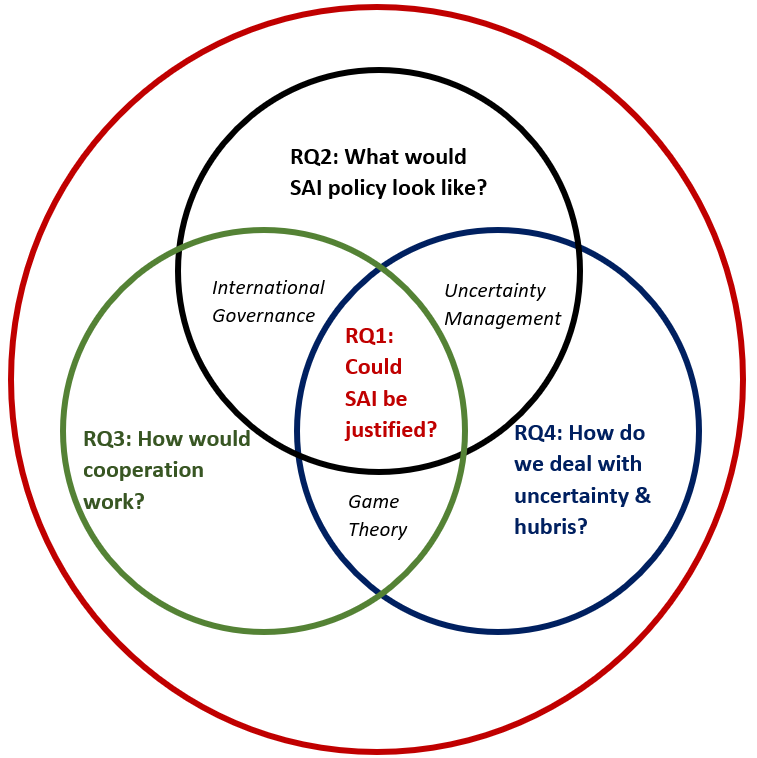
\includegraphics[width=0.7\textwidth]{ThesisMap2.PNG}
    \caption{Conceptual map of thesis scope and research question interlinkages.}
    \label{fig:thesisMap}
\end{figure}

\end{enumerate}

%Question of hubris (much broader - to do with scientific knowledge, uncertainty, confidence and complexity) 

%Write what I have in mind now, doesn't need to be fully specified papers
%Associate HDR Director (Phil G) - research gap needs to be clear and plausible publishability

\section*{Topic 1: Conditions for justifiable deployment}
\label{Topic1}
For this topic I will examine the primary concerns around SAI, and their responses, in order to make the argument that deployment could be ethically justifiable in plausible near-future scenarios. In particular, this introductory work will synthesize an interdisciplinary stance on these issues, which outlines failure modes for deployment, and notable outstanding challenges in scientific uncertainty \citep{kravitz2020uncertainty} and international governance \citep{reynolds2019solar} that need to be addressed as part of ongoing research. As such, the conclusion of this work will describe some conditions an SAI deployment package would need to meet in order to satisfy justifiable use.

In order to construct this argument, a few particular sub-research questions will be addressed: 

\begin{enumerate}
    \item[\textbf{RQ1.1}] What are the primary objections to SAI research and deployment? How does up-to-date research on side-effects and impacts stack up against these concerns?
    \item[\textbf{RQ1.2}] What are conditions for legitimate international governance that would address major governance-based objections?
    \item[\textbf{RQ1.3}] Considering the scientific research on potential SAI impacts, and plausibility of legitimate governance simultaneously, would such a deployment package satisfy ethical requirements?

\end{enumerate}

The paper for this topic, which is currently being drafted and planned for submission to Climatic Change, aims to have a distinctly interdisciplinary approach in synthesizing both scientific (climate, atmospheric physics \& chemistry, impacts modelling) and governance literature on the topic of SAI. In part, this paper is additionally aimed as a response to critical articles such as \cite{pierrehumbert2019there} and \cite{robock200820}.
 
The synthesis in the paper addresses many of the outstanding controversial issues surrounding SAI, clarifying which issues and side-effects are legitimate and still uncertain, and which may be properly addressed with adequate governance and deployment implementation. \medskip

If the governance arrangement is legitimate, just and democratic, then the decision to deploy based on agreed epistemic preconditions is by definition justifiable. Whilst there will always be uncertainty of some kind, if it is approached from legitimate governance, then choices made under such uncertainty are intrinsically politically justifiable. Nevertheless, investigating the details of how this could operate based on current literature is a significant aspect of this topic.\medskip

Finally, it is vital to not lose sight of ethical questions and ramifications in such discussions of SAI. As such, the paper addressing \textbf{RQ1} will endeavour to apply an ethical lens throughout, including several sub-sections on the ethical dimensions of assessing side-effects and procedural justice for legitimate governance. \medskip

Given the overlaps of research questions as described in Figure \ref{fig:thesisMap}, I intend this first paper to only be a ``first pass'' on the topic of justifiable deployment, later returning to the question at the end of the thesis after having considered \textbf{RQs 2 --- 4}. As such, \textbf{RQ1} serves as both an introduction and conclusion to this thesis as a whole.
%The way uncertainty has been managed is politically justified. 
%Justice element
%Decision rules themselves deal with uncertainty, it does not need to be eliminated
\clearpage
\section*{Topic 2: Exploring the optimal climate policy mix with SAI}
\label{Topic2}

The second major topic for this thesis is about exploring scenarios of optimal policy mix of mitigation, adaptation, carbon dioxide removal and solar geoengineering within an integrated assessment model. Through discussions with IAM modelling experts at European Institute on Economics and the Environment (EIEE), I concluded that the RICE50+ \citep{RICE} and WITCH models \citep{emmerling2016witch} developed by EIEE  would be adequate for both \textbf{RQ2} and \textbf{RQ3}. Both these models run using the modelling software GAMS \citep{GAMS}, which I have now acquired an academic license for.\medskip

My first foray into modelling optimal climate policy will be done using RICE50+ given its relative simplicity and low computational requirement. The fast runtime of the model (seconds --- minutes on personal laptop) will allow for rapid turnaround in debugging and scenario experimentation. After the modelling has been finalized and a paper for this topic is underway, I will then consider whether or not extending the work using the more complex WITCH IAM would be appropriate, or whether to move on to the third topic just using RICE50+. Along the way, I will seek advice and expert help with the WITCH team at EIEE as necessary.\medskip

A significant contribution this work would result in is exploring how optimal climate policy scenarios with a solar geoengineering policy option available can be modelled using cost-effectiveness analysis (CEA). This significantly departs from traditional approaches of cost-benefit analysis (CBA), but would avoid inbuilt moral hazard concerns without use of unjustified climate damage functions. Use of CEA with regional optimization and SAI will require careful set up of the decision-problem and solution algorithm to resolve intrinsic difficulties when considering regional optimization. \medskip

Finally, consideration of deep uncertainty in scenario formulation and model analysis will be a significant focus of this topic. Choice of deep uncertainty method(s) for this research is currently underway. Choice of methodology here is a non-trivial problem, since traditionally IAM research has had poor treatment of deep uncertainty so there is very little guidelines on best practice from IAM studies to operate from. Ultimately, management of deep uncertainty will likely take the form of explicitly addressing scenario uncertainty \citep{elsawah2020scenario}, and comprehensive sensitivity analysis of RICE50+, using modern methods \citep{saltelli2008global}. Listed below are some (tentative) specific research questions that summarise the focus of Topic 2.

\begin{enumerate}
    \item[\textbf{RQ2.1}] How does the availability of SAI as a policy option alter optimal climate policy in RICE50+?
    \item[\textbf{RQ2.2}] How does the climate policy mix with SAI change when using cost-effectiveness instead of cost-benefit analysis?
    \item[\textbf{RQ2.3}] What are the major sources of (deep) uncertainty in such climate policy simulations in the context of SAI, and can careful use of scenarios overcome such uncertainty?
\end{enumerate}
In this case, \textbf{RQ2.1} and \textbf{RQ2.2} may be addressed in one paper, whilst \textbf{RQ2.3} may well justify a separate paper for publication. I would aim to publish this modelling work in Environmental Modelling and Software and/or Environmental Resource Economics. \clearpage

\section*{Topic 3: Plausible Scenarios for Semi-Cooperative Solar Geoengineering}

The third topic focuses on cooperation dynamics, and will also utilise an IAM framework through the WITCH model, which implements strategic interactions. The primary goal of this topic will be to explore and model plausible scenarios, such as particular configurations of cooperative coalitions, and testing viable paths to cooperative behaviour when a non-cooperative context is assumed. As such, investigating this topic will draw from game theory and coalition formation studies, both of which have a long history in climate research more broadly \citep{carraro1993strategies}. Moreover, the generation of plausible scenarios will necessarily draw from deep uncertainty methods \citep{elsawah2020scenario,kwakkel2013exploratory} and possibly broader international relations \& governance literature \citep{reynolds2019solar}. For this latter element (which I have less familiarity with), I plan to confer with expert scholars in solar geoengineering research as necessary. \medskip

The following sub-questions outline the scope of this topic:

\begin{enumerate}
    \item[\textbf{RQ3.1}] What possible future incentive structures might lead to unilateral, minilateral or multilateral deployment?
    \item[\textbf{RQ3.2}] Given some representative geopolitical scenarios and coalition formation rules, how does climate policy play out in a non-cooperative setting?
    \item[\textbf{RQ3.3}] Is cooperation plausible across different governance scenarios?
\end{enumerate}

I am currently in discussion with Andrew Lockley and Peter Irvine planning a highly relevant paper to Topic 3, looking at the incentive structure for unilateral/minilateral deployment of SAI. My planned contribution to this collaborative paper would be to put together the game-theoretic formulation and analyse the conceptual model. The same formulation and work will feed quite neatly into my planned thesis work for \textbf{RQ3}. Depending on the extent of my contribution, the resulting collaborative paper may be included in the thesis. \medskip

The paper(s) associated with Topic 3 would be geared towards publication in journals such as Environmental Resources and Economics, Ecological Economics or Environmental Research Letters, all of which have previously published similar game-theoretic work on SAI previously.
\clearpage
\section*{Topic 4: Hubris and Uncertainty}
Whilst the above three topics do tackle uncertainty obliquely, the purpose of Topic 4 is to tackle the concomitant ethical question of hubris within a distinct context of scientific uncertainty. Ultimately, how we make choices in the face of uncertainty through integrated assessment modelling and policy scenarios may or may not be justified, particularly given controversies around IAMs \citep{pindyck2013climate,keen2020appallingly,pezzey2019social}. Understanding the epistemic basis for sound decisions under uncertainty is of vital ethical importance for considering solar geoengineering \citep{NAP2021}. \medskip

Given the wealth of previous work in philosophy of science \citep{carnap2012introduction}, ethics \citep{tannert2007ethics}, socio-epistemology \citep{morrison2021models} and decision making under deep uncertainty \citep{marchau2019decision}, there is much to draw from. Although relatively little philosophical work has treated the problem of hubris extensively, much attention has been placed on the counterpart; intellectual humility \citep{church2016doxastic,hazlett2012higher}, which may provide a sound basis from which to start from. 
Some work looking at the perspective of climate modelling has already begun explicitly tackling questions of uncertainty and decision making \citep{helgeson2020structuring, hill2016climate}. \medskip

From this background literature, I would hope to elucidate under what conditions a choice to deploy SAI may be justified despite uncertainty, or when such a choice could be rightly regarded as ``hubristic'' and ought to be avoided. My work on this topic would thus be explicitly normative. \medskip

As this last research topic has yet to be fully scoped out, the following summary questions are as yet highly tentative.

\begin{enumerate}
    \item[\textbf{RQ4.1}] What is an appropriate conception of ``hubris'' which incorporates scientific and deep uncertainty?
    \item[\textbf{RQ4.2}] Under what conditions would the decision to deploy SAI qualify as hubristic, or not?
    \item[\textbf{RQ4.3}] How can governance of research and development proceed in a way that avoids pitfalls of epistemic arrogance and hubris?
\end{enumerate}

Depending on the precise framing of the related paper(s), the publication could be geared towards a philosophy of science journal such as Synthese, or an interdisciplinary modelling journal such as Earth's Future. I expect to collaborate with an academic in a relevant discipline (e.g. philosophy of science) and have begun discussions with potential co-authors.
\clearpage
%Arctic deployment
\section*{Thesis Plan}
%Key Milestones/checkpoints
%Specific about particular date, but not that "X must be done by that date" rather "At Y date, I will check xyz"
%Double as annual goals
%Fixed timeframe, variable scope
%and the so-what, plus contingency plan in a broad perspective, adaptive planning
Given the transdisciplinary nature of this thesis along with the complex and rapidly evolving context of climate change and solar geoengineering, it seems more appropriate to set the plan for this thesis based on milestones which define a fixed timeframe but variable scope. To safeguard against possible issues, I'll also detail contingency plans to allow for adaptive changes to research questions and planned papers.

\begin{itemize}
    \item[\textbf{May 2021}] Aim for completion and submission of first paper to Climatic Change. If not met, drop other commitments and finish paper ASAP.
    \item[\textbf{July 2021}] Check computer modelling progress with Topic 2, and refine scope as necessary.
    \item[\textbf{September 2021}] Check progress with scoping \& literature review for Topic 3. If path forward unclear or significant computational difficulties arise with WITCH, collapse Topic 3 into Topic 2 and focus on using RICE50+.
    \item[\textbf{October 2021}] If working on collaboration(s) with international colleagues on thesis-relevant paper(s), check progress on such projects and re-evaluate workload as necessary. 
    \item[\textbf{November 2021}] Review progress on thesis with panel and set milestone dates for 2022
    \item[\textbf{February 2022}] Mid term review --- aim to have Topic 2 and collaborative projects from 2021 wrapped up (submitted or ready to submit)
    \item[\textbf{July 2022}] Check progress with Topic 3, refine as necessary
    \item[\textbf{November 2022}] Review progress with panel, set milestones for 2023
    \item[\textbf{March 2023}] Check progress with Topic 4. Aim to be underway with thesis writing
    \item[\textbf{August 2023}] Final Oral Presentation
    \item[\textbf{September 2023}] Determine if six month extension necessary
    \item[\textbf{February 2024}] Thesis Submission (August 2024 with extension)
\end{itemize}

The above dates and additional milestones are open to suggestions by the panel.

\subsection*{Additional Contingencies}
Depending on speed of progress, a number of alternative pathways can be taken to ensure sufficient publications are completed for this thesis. If workload and time management is the primary issue, I can reduce or eliminate other obligations as necessary.\medskip

If by Mid-Late 2021 insufficient progress has been made on Topics 1 - 3, I can also leverage the opportunity to collaborate with colleagues working on similar projects:

\begin{itemize}
    \item Social network analysis and text mining of public sentiment of solar geoengineering on Twitter with Prof. Jan Minx (Mercator Research Institute on Global Commons and Climate Change, Germany) --- I have previous experience with such work, project is well defined
    \item Improving SAI implementation in RICE50+ (or WITCH) with Johannes Emmerling (EIEE, Italy) --- highly restricted scope alternative for Topic 2, previously discussed with Dr. Emmerling
    \item Game-theoretic model of hegemonic solar geoengineering deployment with Andrew Lockley and Peter Irvine --- Scope of project already determined
    \item Politically relevant solar geoengineering 
\end{itemize}

Outside of collaborations, alternative publications could be focused on if deemed more tractable:

\begin{itemize}
    \item Review of uncertainty management in solar geoengineering research
    \item SAI impact assessment on hydrology in Australia using downscaled climate model data from Geoengineering Model Intercomparison Project
    \item Qualitative scenario exploration for SAI (e.g. workshop based)
    \item Sensitivity analysis of semi-empirical damage functions for SAI in RICE50+
\end{itemize}

\section*{Summary of Contribution}
Overall, this thesis aims to produce policy-relevant, transdisciplinary knowledge which can enable more effective decision making in the future regarding solar geoengineering. Addressing \textbf{RQ1} on whether SAI is conceivably justifiable will be both the start and culmination of this work, and although not the last word on the matter, I hope my contribution to the literature on such a pertinent question will ultimately spur further work on SAI, whilst providing an updated foundation for public and academic discussions. \medskip

More specifically, addressing \textbf{RQ2} and \textbf{RQ3} regarding optimal climate policy and cooperative deployment will help shed light on crucial questions of governance, giving more epistemic confidence to would-be geoengineers about how to begin strategizing towards a better possible future. Exploration of climate policy scenarios within an integrated assessment model framework will also help pave the path towards mainstream consideration of SAI policy, hopefully through future IPCC assessment reports. \medskip

Investigating issues of uncertainty and hubris for \textbf{RQ4} will also help build a more solid ethical foundation for future decision-making around SAI. In particular, specifying necessary criteria for when too much uncertainty poses ethically significant risks could aid in the construction of regulatory and governance norms around solar geoengineering. \medskip

Finally, throughout all this work I am and will continue to endeavour to collaborate with other researchers across various disciplines working on similar questions on SAI. The growth of a collaborative and internationally diverse research community is critical in advancing solar geoengineering research and governance. By playing a small role in this process, I hope that my thesis work will contribute not just to academic knowledge but wider efforts towards a hopeful future.

\clearpage

\bibliographystyle{plainnat}
\bibliography{biblio}

\end{document}
